%  LaTeX support: latex@mdpi.com 
%  For support, please attach all files needed for compiling as well as the log file, and specify your operating system, LaTeX version, and LaTeX editor.

%=================================================================
\documentclass[atmosphere,article,submit,moreauthors]{Definitions/mdpi} 
% For posting an early version of this manuscript as a preprint, you may use "preprints" as the journal and change "submit" to "accept". The document class line would be, e.g., \documentclass[preprints,article,accept,moreauthors,pdftex]{mdpi}. This is especially recommended for submission to arXiv, where line numbers should be removed before posting. For preprints.org, the editorial staff will make this change immediately prior to posting.

%--------------------
% Class Options:
%--------------------
%----------
% journal
%----------
% Choose between the following MDPI journals:
% acoustics, actuators, addictions, admsci, adolescents, aerospace, agriculture, agriengineering, agronomy, ai, algorithms, allergies, alloys, analytica, animals, antibiotics, antibodies, antioxidants, applbiosci, appliedchem, appliedmath, applmech, applmicrobiol, applnano, applsci, aquacj, architecture, arts, asc, asi, astronomy, atmosphere, atoms, audiolres, automation, axioms, bacteria, batteries, bdcc, behavsci, beverages, biochem, bioengineering, biologics, biology, biomass, biomechanics, biomed, biomedicines, biomedinformatics, biomimetics, biomolecules, biophysica, biosensors, biotech, birds, bloods, blsf, brainsci, breath, buildings, businesses, cancers, carbon, cardiogenetics, catalysts, cells, ceramics, challenges, chemengineering, chemistry, chemosensors, chemproc, children, chips, cimb, civileng, cleantechnol, climate, clinpract, clockssleep, cmd, coasts, coatings, colloids, colorants, commodities, compounds, computation, computers, condensedmatter, conservation, constrmater, cosmetics, covid, crops, cryptography, crystals, csmf, ctn, curroncol, currophthalmol, cyber, dairy, data, dentistry, dermato, dermatopathology, designs, diabetology, diagnostics, dietetics, digital, disabilities, diseases, diversity, dna, drones, dynamics, earth, ebj, ecologies, econometrics, economies, education, ejihpe, electricity, electrochem, electronicmat, electronics, encyclopedia, endocrines, energies, eng, engproc, ent, entomology, entropy, environments, environsciproc, epidemiologia, epigenomes, est, fermentation, fibers, fintech, fire, fishes, fluids, foods, forecasting, forensicsci, forests, foundations, fractalfract, fuels, futureinternet, futureparasites, futurepharmacol, futurephys, futuretransp, galaxies, games, gases, gastroent, gastrointestdisord, gels, genealogy, genes, geographies, geohazards, geomatics, geosciences, geotechnics, geriatrics, hazardousmatters, healthcare, hearts, hemato, heritage, highthroughput, histories, horticulturae, humanities, humans, hydrobiology, hydrogen, hydrology, hygiene, idr, ijerph, ijfs, ijgi, ijms, ijns, ijtm, ijtpp, immuno, informatics, information, infrastructures, inorganics, insects, instruments, inventions, iot, j, jal, jcdd, jcm, jcp, jcs, jdb, jeta, jfb, jfmk, jimaging, jintelligence, jlpea, jmmp, jmp, jmse, jne, jnt, jof, joitmc, jor, journalmedia, jox, jpm, jrfm, jsan, jtaer, jzbg, kidney, kidneydial, knowledge, land, languages, laws, life, liquids, literature, livers, logics, logistics, lubricants, lymphatics, machines, macromol, magnetism, magnetochemistry, make, marinedrugs, materials, materproc, mathematics, mca, measurements, medicina, medicines, medsci, membranes, merits, metabolites, metals, meteorology, methane, metrology, micro, microarrays, microbiolres, micromachines, microorganisms, microplastics, minerals, mining, modelling, molbank, molecules, mps, msf, mti, muscles, nanoenergyadv, nanomanufacturing, nanomaterials, ncrna, network, neuroglia, neurolint, neurosci, nitrogen, notspecified, nri, nursrep, nutraceuticals, nutrients, obesities, oceans, ohbm, onco, oncopathology, optics, oral, organics, organoids, osteology, oxygen, parasites, parasitologia, particles, pathogens, pathophysiology, pediatrrep, pharmaceuticals, pharmaceutics, pharmacoepidemiology, pharmacy, philosophies, photochem, photonics, phycology, physchem, physics, physiologia, plants, plasma, pollutants, polymers, polysaccharides, poultry, powders, preprints, proceedings, processes, prosthesis, proteomes, psf, psych, psychiatryint, psychoactives, publications, quantumrep, quaternary, qubs, radiation, reactions, recycling, regeneration, religions, remotesensing, reports, reprodmed, resources, rheumato, risks, robotics, ruminants, safety, sci, scipharm, seeds, sensors, separations, sexes, signals, sinusitis, skins, smartcities, sna, societies, socsci, software, soilsystems, solar, solids, sports, standards, stats, stresses, surfaces, surgeries, suschem, sustainability, symmetry, synbio, systems, taxonomy, technologies, telecom, test, textiles, thalassrep, thermo, tomography, tourismhosp, toxics, toxins, transplantology, transportation, traumacare, traumas, tropicalmed, universe, urbansci, uro, vaccines, vehicles, venereology, vetsci, vibration, viruses, vision, waste, water, wem, wevj, wind, women, world, youth, zoonoticdis 

%---------
% article
%---------
% The default type of manuscript is "article", but can be replaced by: 
% abstract, addendum, article, book, bookreview, briefreport, casereport, comment, commentary, communication, conferenceproceedings, correction, conferencereport, entry, expressionofconcern, extendedabstract, datadescriptor, editorial, essay, erratum, hypothesis, interestingimage, obituary, opinion, projectreport, reply, retraction, review, perspective, protocol, shortnote, studyprotocol, systematicreview, supfile, technicalnote, viewpoint, guidelines, registeredreport, tutorial
% supfile = supplementary materials

%----------
% submit
%----------
% The class option "submit" will be changed to "accept" by the Editorial Office when the paper is accepted. This will only make changes to the frontpage (e.g., the logo of the journal will get visible), the headings, and the copyright information. Also, line numbering will be removed. Journal info and pagination for accepted papers will also be assigned by the Editorial Office.

%------------------
% moreauthors
%------------------
% If there is only one author the class option oneauthor should be used. Otherwise use the class option moreauthors.

%---------
% pdftex
%---------
% The option pdftex is for use with pdfLaTeX. If eps figures are used, remove the option pdftex and use LaTeX and dvi2pdf.

%=================================================================
% MDPI internal commands
\firstpage{1} 
\makeatletter 
\setcounter{page}{\@firstpage} 
\makeatother
\pubvolume{1}
\issuenum{1}
\articlenumber{0}
\pubyear{2022}
\copyrightyear{2022}
%\externaleditor{Academic Editor: Firstname Lastname} % For journal Automation, please change Academic Editor to "Communicated by"
\datereceived{} 
\dateaccepted{} 
\datepublished{} 
%\datecorrected{} % Corrected papers include a "Corrected: XXX" date in the original paper.
%\dateretracted{} % Corrected papers include a "Retracted: XXX" date in the original paper.
\hreflink{https://doi.org/} % If needed use \linebreak
%\doinum{}
%------------------------------------------------------------------
% The following line should be uncommented if the LaTeX file is uploaded to arXiv.org
%\pdfoutput=1

%=================================================================
% Add packages and commands here. The following packages are loaded in our class file: fontenc, inputenc, calc, indentfirst, fancyhdr, graphicx, epstopdf, lastpage, ifthen, lineno, float, amsmath, setspace, enumitem, mathpazo, booktabs, titlesec, etoolbox, tabto, xcolor, soul, multirow, microtype, tikz, totcount, changepage, attrib, upgreek, cleveref, amsthm, hyphenat, natbib, hyperref, footmisc, url, geometry, newfloat, caption
\usepackage{pdflscape}
\usepackage{siunitx}
\usepackage{aas_macros}
\usepackage{etoolbox}
\usepackage{fixltx2e}
%=================================================================
%% Please use the following mathematics environments: Theorem, Lemma, Corollary, Proposition, Characterization, Property, Problem, Example, ExamplesandDefinitions, Hypothesis, Remark, Definition, Notation, Assumption
%% For proofs, please use the proof environment (the amsthm package is loaded by the MDPI class).

%=================================================================
% Full title of the paper (Capitalized)
\Title{Title}

% MDPI internal command: Title for citation in the left column
\TitleCitation{Title}

% Author Orchid ID: enter ID or remove command
\newcommand{\orcidauthorA}{0000-0000-0000-000X} % Add \orcidA{} behind the author's name
%\newcommand{\orcidauthorB}{0000-0000-0000-000X} % Add \orcidB{} behind the author's name

% Authors, for the paper (add full first names)
\Author{Jorge Tarango-Yong $^{1,\dagger,\ddagger}$\orcidA{}, Mario Rodr\'iguez-Mart\'inez $^{1,\ddagger}$ and Raul Guti\'errez-Zalapa $^{2,}$*}

%\longauthorlist{yes}

% MDPI internal command: Authors, for metadata in PDF
\AuthorNames{Jorge Tarango-Yong, Mario Rodr\'iguez-Mart\'inez and Raul Guti\'errez-Zalapa}

% MDPI internal command: Authors, for citation in the left column
\AuthorCitation{Tarango-Yong, J.; Rodr\'iguez-Mart\'inez, M.; Guti\'errez-Zalapa, R.}
% If this is a Chicago style journal: Lastname, Firstname, Firstname Lastname, and Firstname Lastname.

% Affiliations / Addresses (Add [1] after \address if there is only one affiliation.)
\address{%
$^{1}$ \quad Affiliation 1; e-mail@e-mail.com\\
$^{2}$ \quad Affiliation 2; e-mail@e-mail.com}

% Contact information of the corresponding author
\corres{Correspondence: e-mail@e-mail.com; Tel.: (optional; include country code; if there are multiple corresponding authors, add author initials) +xx-xxxx-xxx-xxxx (F.L.)}

% Current address and/or shared authorship
\firstnote{Current address: Affiliation 3} 
\secondnote{These authors contributed equally to this work.}
% The commands \thirdnote{} till \eighthnote{} are available for further notes

%\simplesumm{} % Simple summary

%\conference{} % An extended version of a conference paper

% Abstract (Do not insert blank lines, i.e. \\) 
\abstract{A single paragraph of about 200 words maximum. For research articles, abstracts should give a pertinent overview of the work. We strongly encourage authors to use the following style of structured abstracts, but without headings: (1) Background: place the question addressed in a broad context and highlight the purpose of the study; (2) Methods: describe briefly the main methods or treatments applied; (3) Results: summarize the article's main findings; (4) Conclusion: indicate the main conclusions or interpretations. The abstract should be an objective representation of the article, it must not contain results which are not presented and substantiated in the main text and should not exaggerate the main conclusions.}

% Keywords
\keyword{keyword 1; keyword 2; keyword 3 (List three to ten pertinent keywords specific to the article; yet reasonably common within the subject discipline.)} 

% The fields PACS, MSC, and JEL may be left empty or commented out if not applicable
%\PACS{J0101}
%\MSC{}
%\JEL{}

%%%%%%%%%%%%%%%%%%%%%%%%%%%%%%%%%%%%%%%%%%
% Only for the journal Diversity
%\LSID{\url{http://}}

%%%%%%%%%%%%%%%%%%%%%%%%%%%%%%%%%%%%%%%%%%
% Only for the journal Applied Sciences:
%\featuredapplication{Authors are encouraged to provide a concise description of the specific application or a potential application of the work. This section is not mandatory.}
%%%%%%%%%%%%%%%%%%%%%%%%%%%%%%%%%%%%%%%%%%

%%%%%%%%%%%%%%%%%%%%%%%%%%%%%%%%%%%%%%%%%%
% Only for the journal Data:
%\dataset{DOI number or link to the deposited data set in cases where the data set is published or set to be published separately. If the data set is submitted and will be published as a supplement to this paper in the journal Data, this field will be filled by the editors of the journal. In this case, please make sure to submit the data set as a supplement when entering your manuscript into our manuscript editorial system.}

%\datasetlicense{license under which the data set is made available (CC0, CC-BY, CC-BY-SA, CC-BY-NC, etc.)}

%%%%%%%%%%%%%%%%%%%%%%%%%%%%%%%%%%%%%%%%%%
% Only for the journal Toxins
%\keycontribution{The breakthroughs or highlights of the manuscript. Authors can write one or two sentences to describe the most important part of the paper.}

%%%%%%%%%%%%%%%%%%%%%%%%%%%%%%%%%%%%%%%%%%
% Only for the journal Encyclopedia
%\encyclopediadef{Instead of the abstract}
%\entrylink{The Link to this entry published on the encyclopedia platform.}
%%%%%%%%%%%%%%%%%%%%%%%%%%%%%%%%%%%%%%%%%%
\begin{document}

%%%%%%%%%%%%%%%%%%%%%%%%%%%%%%%%%%%%%%%%%%
%\setcounter{section}{-1} %% Remove this when starting to work on the template.
%\section{How to Use this Template}

%The template details the sections that can be used in a manuscript. Note that the order and names of article sections may differ from the requirements of the journal (e.g., the positioning of the Materials and Methods section). Please check the instructions on the authors' page of the journal to verify the correct order and names. For any questions, please contact the editorial office of the journal or support@mdpi.com. For LaTeX-related questions please contact latex@mdpi.com.%\endnote{This is an endnote.} % To use endnotes, please un-comment \printendnotes below (before References). Only journal Laws uses \footnote.

% The order of the section titles is: Introduction, Materials and Methods, Results, Discussion, Conclusions for these journals: aerospace,algorithms,antibodies,antioxidants,atmosphere,axioms,biomedicines,carbon,crystals,designs,diagnostics,environments,fermentation,fluids,forests,fractalfract,informatics,information,inventions,jfmk,jrfm,lubricants,neonatalscreening,neuroglia,particles,pharmaceutics,polymers,processes,technologies,viruses,vision


\section{Introduction}
%The Earth's magnetic field represents a final obstacle to the Solar Wind (SW) flux. When descelerated and defected by a non colisional shock wave in the flux direction, generates a cavity known as magnetosphere \citep{Blanco-Cano:2004}. Since the Earth is embedded in this SW flux, is known that under adequated physical conditions (e.g magnetic reconnection) may exist some coupling between the magnetosphere and the Earth's ionosphere \citep{Zolesi:2014, Cnossen:2014}.

The Sun plays an important role in the physical proccesses that occur in the terrestrial magnetosphere-ionosphere system. When the SW interacts with the Earth's magnetosphere, particles may permeate the internal region via magnetic reconnection and penetrate to polar zones and generate boreal or austral auroras thus altering the system \citep{Vazquez:2016, Oka:2011}. By the other hand, the Extreme Ultraviolet Radiation (EUV) and X-rays coming from the Sun may interact with the neutral atmoshere via photoionization \citep{Vlasov:2010}. However, in both cases the final result is that the ionosphere's free electrons population is altered.

Some Ionospheric Perturbations (IP) become relevant due to their spatial and temporal scale in the Space Weather scenario. At intermediate latitudes, the most common in the ionosphere are known as Traveling Ionospheric Disturbances (TIDs). Typically they divide into two groups: a) large scale TIDs, associated with geomagnetic storms with sizes of \SI{\sim 2000}{km}, periods of \SI{\sim 1}{h} and velocities of \SI{\sim 700}{km.s^{-1}}, and b) Medium-scale TIDs, which are not fully associated with geomagnetic storms, present sizes of \SI{\sim 100}{km}, periods from 10 minutes to 1 hour and velocities between \SI{50}{km.s^{-1}} and \SI{1e2}{km.s^{-1}} \citep{Helmboldt:2012}. Diverse methods have benn used to study TIDs, such as incoherent dispersion radars, high frequency Doppler emmisors, data from Global Positioning System (GPS) stations or even radiotelescopes like the VLA or the Mexican Array Radio Telescope (MEXART) \citep{Chilcote:2015, Rodriguez:2014}.

On the other side, the Earth's ionosphere may be affected or modified by other proccesses, particularly there are studies that show how the Vetical Total Electron Content (vTEC) due to shock waves generated for rockets launched to space \citep{Lin:2014}. Similar proccesses modify the Earth's ionosphere due to objects entering the athmosphere from space, such as meteoroids like the one which fell on Chelyabinsk at 2013 \citep{Yang:2014}. Previously, the ionospheric perturbations produced by this object were studied using two independent methods: a) detecting vTEC pertubations using GPS station near the impact location. And b) a wavelets analysis for detection of ...

In 2020 a meteoroid passed in mexican territory through mexican territory, which also was studied \citep{Sergeeva:2020}. The meteoroid was recorded with outdoor cameras in different locations. The trajectory could be estimated, as well as other physical parameters.

In this work we will show a similar analysis for a sample of meteoroids detected in mexican territory by different methods. The first subsample consists in objects detected by the Geostationary Lightning Mapper (GLM) whose sizes are estimated between a few decimeters to meters in diameter \citep{GOODMAN:2013, Jenniskens:2018, Rumpf:2019}. The second subsample will consist in objects detected by ocular witnesses from the American Meteor Society and as comparisson we will include the morelian meteoroid reported in \citet{Sergeeva:2020} and the Chelyabinsk event \citet{Yang:2014}. The paper is arranged in the following way: \S \ref{sec:methodology} describes the samples of meteoroids as well of the properties that can be obtained from direct observations. Also describes the GPS data corresponding to the dates and locations where each object was located. \S \ref{sec:bolides} shows physical parameters of meteoroids obtained from the observed heights and energies. Finally, section \S \ref{sec:vTEC-maps} shows the vTEC maps and scintillation indices obtained from GPS observations.  

%The introduction should briefly place the study in a broad context and highlight why it is important. It should define the purpose of the work and its significance. The current state of the research field should be reviewed carefully and key publications cited. Please highlight controversial and diverging hypotheses when necessary. Finally, briefly mention the main aim of the work and highlight the principal conclusions. As far as possible, please keep the introduction comprehensible to scientists outside your particular field of research. Citing a journal paper \cite{ref-journal}. Now citing a book reference \cite{ref-book1,ref-book2} or other reference types \cite{ref-unpublish,ref-communication,ref-proceeding}. Please use the command \citep{ref-thesis,ref-url} for the following MDPI journals, which use author--date citation: Administrative Sciences, Arts, Econometrics, Economies, Genealogy, Humanities, IJFS, Journal of Intelligence, Journalism and Media, JRFM, Languages, Laws, Religions, Risks, Social Sciences, Literature.
%%%%%%%%%%%%%%%%%%%%%%%%%%%%%%%%%%%%%%%%%%
\section{Methodology}
%\subsection{Meteors Databases}
\label{ssec:databases}
We selected a sample of meteors which were observed in mexican territory from the Geostationary Lightning Mapper \citep{GOODMAN:2013}. Orignally this project was designed to detect ligthning activity in earth's athmosphere, but has been proven that also can detect bolides entering the athmosphere. The detection comes from two satellites called GOES-16 and GOES-17 orbiting the earth in geostationary orbits. %Figure  shows the area where GOES-16 and GOES-17 detect activity on a lightning flash rate map; in mexican territory clearly both satellites can make detections. %Create a figure where the area coverage of GOES-16 and GOES-17 is shown.
We used the interactive database available at \url{https://neo-bolide.ndc.nasa.gov/#/}. These data are publicly available and easily downloaded from the same website. For each event we can obtain the recorded trajectory of meteors and the corresponding light curve. THe GLM satellites have an umbral magnitude for detection of -14. At this magnitude, a meteor is considered a bolide, and is expected to be at least decimeter-sized (in diameter) to reach such brightness. In the other hand, too bright meteors will saturate the detectors, and thus, lowering the quality of data. The result of this factors implies that the range in size of the objects in our sample varies in diameter between decimeter to meter size. %The sample was chosen following the next criteria:%selected in such way we chose the most probable objects to be detected by GPS sources in mexican territory and its surroundings: 
Each event also has assigned a confidence ratio, from low confidence to high, depending in how bright is the event itself and if the trajectory recorded by GLM ressembles (or not) a straight line. We chose only events whose confidence ratio is high, in oreder to be sure we chose the brightest objects, and thus, in the diameter size of bolides, we favored the meter-sized ones. In table \ref{tab:table-meteors} we list the object we chose to do this work, order in chronological order. The columns of the table, from left to right are and ID to enumerate the meteors in the sample, the date and time each meteor was detected, the duration of the detection, their respective coordinates and the estimated height of the meteor over the ground at the time of the detection. GOES-16 and GOES-17 systematically detect the meteors at slightly different positions and at slightly different times, so we calculated the mean of the duration, latitude and longitude reported by both satellites for each event, and used the standard deviation as the uncertainties.

From table \ref{tab:table-meteors} is also clear that the duration of all the bolides detection last less than a second. This obsevation suggests that the bolides remain undetected by the GLM satellites until they get fragmented due to stagnation presure when they release a huge amount of energy and thus they become detectable.


%From the light curves we can estimate the total radiated energy and then convert it to the total kinetic energy through a relation. With this energy we may estimate physical parameters with the cloud fragmentation model form wheeler et al.

%\begin{itemize}
%    \item The objects were detected inside mexican territory and its surroundings.
%    \item The objects were detected by both satellites GOES 16 and GOES 17 (stereo)
%    \item The detection has been assigned a high confidence ratio.
%\end{itemize}



\begin{table*}
  \centering
  \footnotesize
  \caption{List of bolides detected in mexican territory (plus one detected near Venezuela and one detected near Cuba), detected by the Geostationary Lighning mapper. The events are listed in chronological order. The listed duration, latitude and longitude correspond to the mean of the measurements of both GOES satellites. The uncertainties correspond to the respecting mean deviation.}
\label{tab:table-meteors}
\begin{tabular}{rrrrrrrrrr}
\hline
ID & Date of event  & Start Time (UT)  & Duration (seconds) & Latitude (deg) & Longitude (deg)& Altitude (km) & Energy (kT )\\\hline
GLM-00 & 2019-02-01 & 18:17:09 & $2.651\pm 0.4907$ & $22.45 \pm 0.071$ & $-83.50  \pm  0.424$ & 24           & 2.0978196 +/- 0.42361329      \\         
GLM-01 & 2019-05-23 & 16:36:18 & $0.197\pm 0.0000$ & $24.30 \pm 0.000$ & $-101.60 \pm  0.849$ & 28           & 0.011954659 +/- 7.4054404e-3  \\
GLM-02 & 2019-07-18 & 14:30:30 & $0.058\pm 0.0000$ & $27.20 \pm 0.000$ & $-103.15 \pm  0.778$ & 72           & 5.7827709e-3 +/- 3.9334336e-3 \\
GLM-03 & 2019-08-10 & 11:18:48 & $0.199\pm 0.0757$ & $21.50 \pm 0.000$ & $-102.50  \pm 0.849$ & 92           & 0.010556123 +/- 6.6488245e-3  \\
GLM-04 & 2019-10-03 & 07:55:33 & $0.106\pm 0.0297$ & $25.65 \pm 0.071$ & $-96.25 \pm   0.778$ & 74           & 2.9915536e-3 +/- 2.2000998e-3 \\
GLM-05 & 2019-10-09 & 06:08:11 & $0.103\pm 0.0078$ & $23.60 \pm 0.000$ & $-111.95 \pm  0.212$ & 32           & 0.021837042 +/- 0.012429732   \\
GLM-06 & 2019-11-16 & 09:36:04 & $0.396\pm 0.0134$ & $20.30 \pm 0.000$ & $-100.55 \pm  0.919$ & 82           & 7.5423706e-3 +/- 4.9626060e-3 \\
GLM-07 & 2019-11-17 & 15:36:01 & $0.116\pm 0.0035$ & $31.70 \pm 0.000$ & $-117.70 \pm  1.131$ & 88           & 0.022397444 +/- 0.012701445   \\
GLM-08 & 2019-11-19 & 07:57:40 & $0.097\pm 0.1138$ & $20.00 \pm 0.000$ & $-88.40 \pm   1.131$ & 99           & 1.5012507e-3 +/- 1.1909667e-3 \\
GLM-09 & 2019-11-26 & 13:23:20 & $0.078\pm 0.0290$ & $23.90 \pm 0.000$ & $-108.70 \pm  0.849$ & 81           & 4.9551290e-3 +/- 3.4345742e-3 \\
GLM-10 & 2019-12-04 & 09:42:54 & $0.173\pm 0.0028$ & $31.50 \pm 0.000$ & $-113.65 \pm  0.919$ & 77           & 0.029149047 +/- 0.015891049   \\
GLM-11 & 2019-12-15 & 14:50:49 & $0.127\pm 0.0134$ & $27.70 \pm 0.000$ & $-114.10 \pm  0.849$ & 78           & 0.010556123 +/- 6.6488245e-3  \\
GLM-12 & 2019-12-29 & 16:16:35 & $0.062\pm 0.0134$ & $29.60 \pm 0.000$ & $-116.35 \pm  0.919$ & 79           & 4.2084911e-3 +/- 2.9746446e-3 \\
GLM-13 & 2020-01-03 & 14:10:17 & $0.113\pm 0.0085$ & $30.20 \pm 0.000$ & $-117.65 \pm  0.919$ & 74           & 0.011607116 +/- 7.2187549e-3  \\
GLM-14 & 2020-01-06 & 16:39:27 & $0.118\pm 0.0042$ & $31.40 \pm 0.000$ & $-108.20 \pm  0.990$ & 81           & 0.015448801 +/- 9.2392402e-3  \\
GLM-15 & 2020-01-15 & 15:00:33 & $0.213\pm 0.1351$ & $19.45 \pm 0.071$ & $-95.55 \pm   0.919$ & 93           & 0.012559739 +/- 7.7284725e-3  \\
GLM-16 & 2020-02-12 & 09:25:40 & $0.210\pm 0.0226$ & $18.90 \pm 0.000$ & $-93.50 \pm   0.849$ & 90           & 8.2107211e-3 +/- 5.3440405e-3 \\
GLM-17 & 2020-03-03 & 12:33:27 & $0.062\pm 0.0007$ & $18.25 \pm 0.071$ & $-106.35 \pm  0.636$ & 77           & 3.4441157e-3 +/- 2.4922397e-3 \\
GLM-18 & 2020-03-31 & 19:31:52 & $0.105\pm 0.0573$ & $28.45 \pm 0.071$ & $-112.05 \pm  0.636$ & 61           & 7.2469897e-3 +/- 4.7924800e-3 \\
GLM-19 & 2020-04-08 & 16:25:28 & $0.120\pm 0.0926$ & $26.10 \pm 0.000$ & $-93.90 \pm   0.849$ & 78           & 4.0292119e-3 +/- 2.8626279e-3 \\
GLM-20 & 2020-04-18 & 17:43:25 & $0.139\pm 0.0106$ & $29.00 \pm 0.000$ & $-106.55 \pm  0.919$ & 82           & 5.8303967e-3 +/- 3.9618242e-3 \\
GLM-21 & 2020-04-20 & 16:05:22 & $0.318\pm 0.1655$ & $28.15 \pm 0.071$ & $-97.85 \pm   1.061$ & 88           & 0.031378060 +/- 0.016913982   \\
GLM-22 & 2020-04-25 & 11:03:09 & $0.323\pm 0.0813$ & $32.15 \pm 0.071$ & $-111.60 \pm  1.131$ & 84           & 0.021997346 +/- 0.012507576   \\
GLM-23 & 2020-04-28 & 19:31:52 & $0.105\pm 0.0573$ & $28.45 \pm 0.071$ & $-112.05 \pm  0.636$ & 29           & 0.12687833 +/- 0.053736010    \\
GLM-24 & 2020-05-08 & 10:06:16 & $0.490\pm 0.0750$ & $21.60 \pm 0.000$ & $-92.40 \pm   0.849$ & 81           & 0.033207253 +/- 0.017743607   \\
GLM-25 & 2020-07-15 & 19:58:28 & $0.693\pm 0.0495$ & $24.00 \pm 0.000$ & $-108.35 \pm  0.495$ & 53           & 0.020548979 +/- 0.011800641   \\
GLM-26 & 2020-08-07 & 13:29:57 & $0.163\pm 0.0057$ & $28.80 \pm 0.000$ & $-106.05 \pm  0.919$ & 89           & 0.014606987 +/- 8.8040841e-3  \\
GLM-27 & 2020-09-13 & 16:41:59 & $0.184\pm 0.0078$ & $28.45 \pm 0.071$ & $-113.75 \pm  0.919$ & 85           & 0.010995616 +/- 6.8881646e-3  \\
GLM-28 & 2020-09-30 & 12:28:11 & $0.100\pm 0.0078$ & $24.90 \pm 0.000$ & $-110.90 \pm  0.849$ & 83           & 0.014013965 +/- 8.4951275e-3  \\
GLM-29 & 2020-11-16 & 12:28:11 & $0.100\pm 0.0078$ & $24.90 \pm 0.000$ & $-110.90 \pm  0.849$ &106           & 0.052044572 +/- 0.025868548   \\
GLM-30 & 2020-11-17 & 12:53:41 & $0.404\pm 0.0262$ & $23.00 \pm 0.000$ & $-102.45 \pm  0.919$ & 93           & 0.060624247 +/- 0.029367156   \\
GLM-31 & 2020-12-19 & 10:18:14 & $0.407\pm 0.0110$ & $21.95 \pm 0.071$ & $-101.60 \pm  0.990$ & 98           & 0.060272985 +/- 0.029225978   \\
GLM-32 & 2020-12-23 & 09:43:01 & $0.148\pm 0.0014$ & $25.75 \pm 0.071$ & $-111.25 \pm  0.778$ & 81           & 0.012127937 +/- 7.4982028e-3  \\
GLM-33 & 2020-12-29 & 15:20:54 & $0.118\pm 0.0014$ & $16.80 \pm 0.000$ & $-102.20 \pm  0.707$ & 81           & 0.013161054 +/- 8.0470909e-3  \\
GLM-34 & 2021-03-31 & 09:01:17 & $0.753\pm 0.3083$ & $20.15 \pm 0.071$ & $-92.95 \pm  0.212$  & 24           & 0.054259119 +/- 0.026782008   \\
GLM-Ven& 2019-06-22 & 21:25:45 & $4.873\pm 0.0000$ & $14.9 \pm 0.000$  & $-65.8 \pm 0.000$    & 25           & 6.1014359 +/- 0.81239700      \\ \hline
\end{tabular}
\end{table*}

\begin{figure}
  \centering
  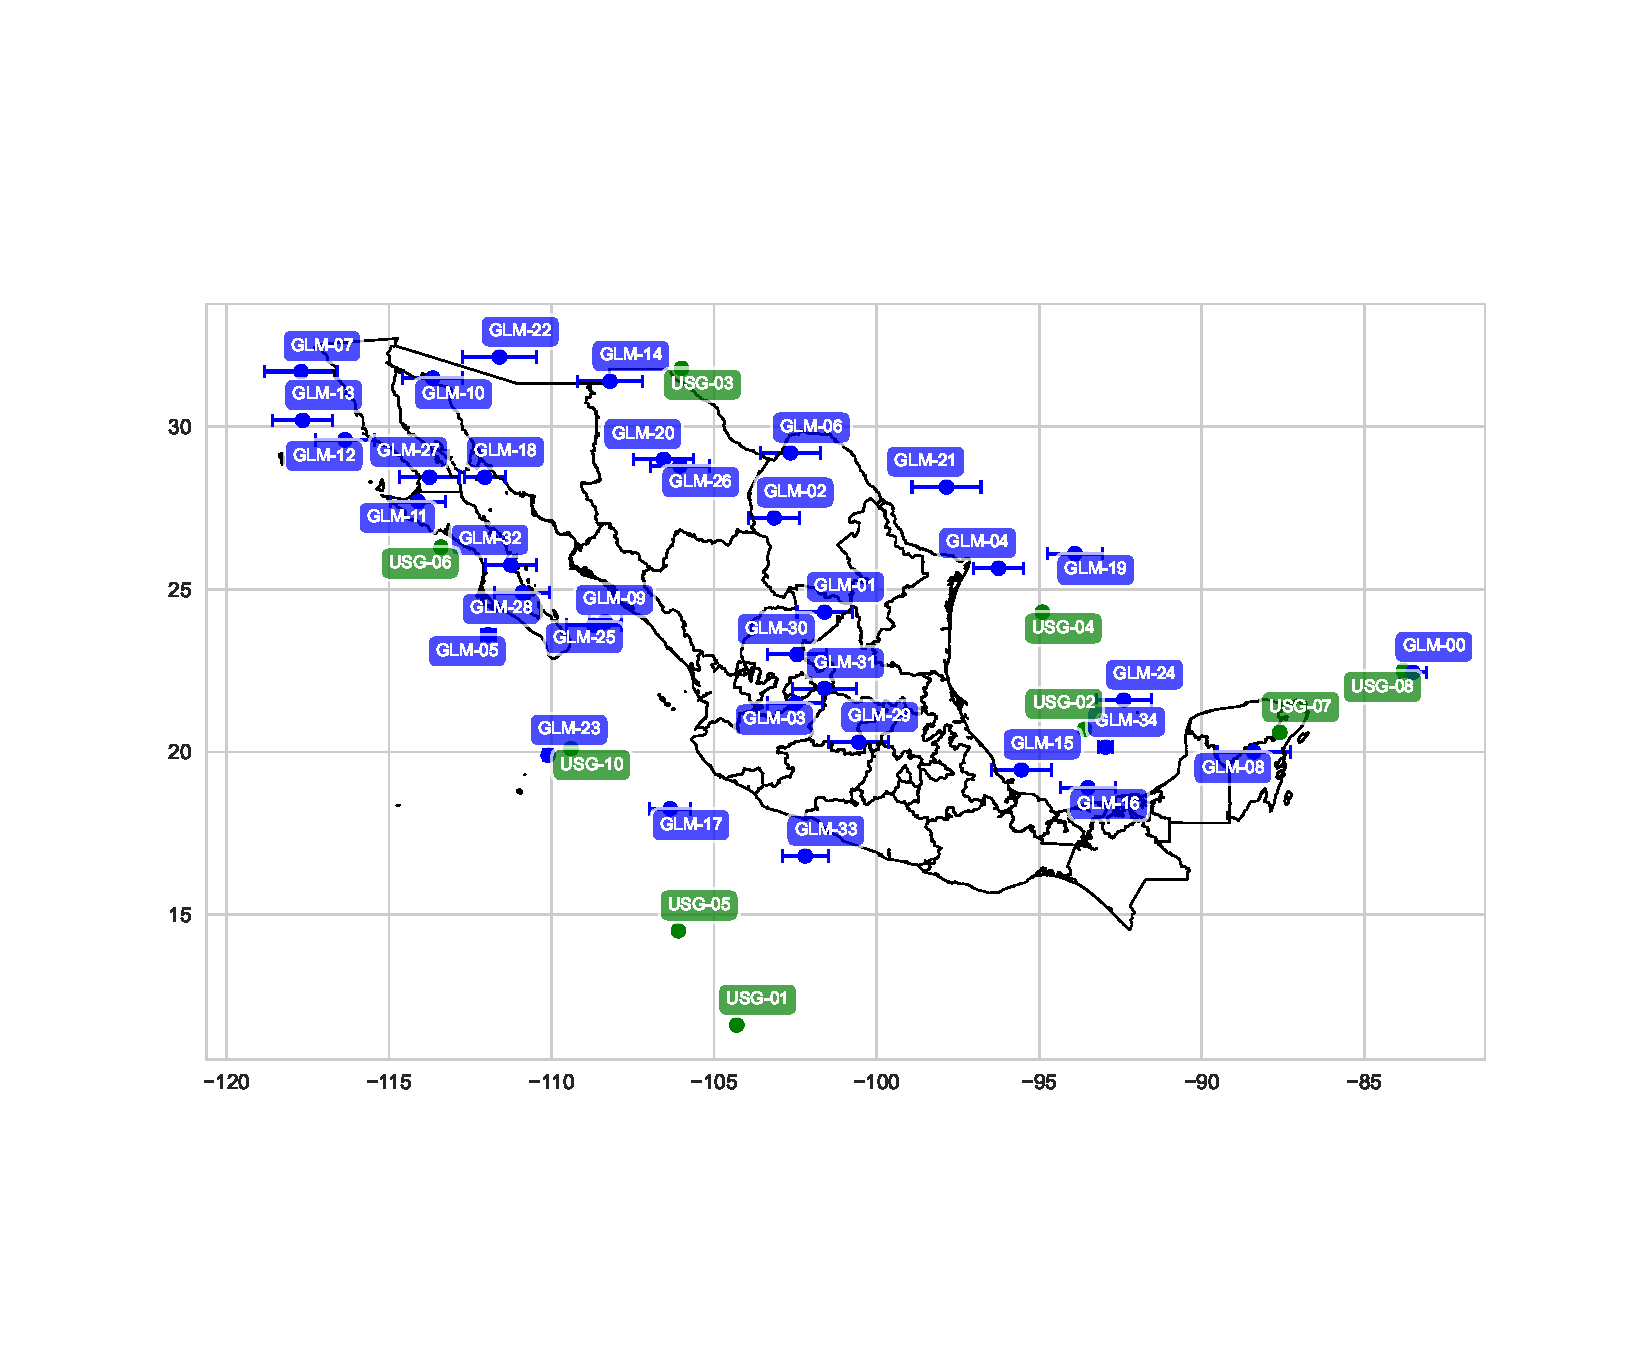
\includegraphics[width=\linewidth]{../meteors_map}
  \caption{Positions of events from table \ref{tab:table-meteors} (blue) and table \ref{tab:table-meteors-2}. The events GLM-00/USG-08 actually correpond to the same bolide, but there are little discrepancies about the position where the bolide was detecte. The same applies for the events GLM-23/USG-10 and GLM-Ven/USG-09, which not appears in the map.}
  \label{fig:meteors-map}
\end{figure}

By the other hand, we got another sample of 10 bolidesfrom US Goverment (USG) sensors from the Center for Near Earth Object Studies (CNEOS), publicly available at \url{https://cneos.jpl.nasa.gov/fireballs/}, where we may obtain directly data about bolides position, the date and time each bolide was detected, the energy released at fragmentation, the velocity and the height (the last two not availble for all bolides). As seen in table \ref{tab:table-meteors-2}, the time span is quite larger, and the released energy is generally larger. Both energy distributions are compared directly in figure \ref{fig:boxplot}. Some elements appear in both samples, since are bright enough to be detected regardless the project involved. In USG sample, the total energy of each meteor is obtained directly, but is not the case for the GLM sample. In appendix \ref{app:distance} and \ref{app:energy} we give details about how this total energy is obtained.

\begin{table*}
    \centering
  \footnotesize
  \caption{List of bolides detected in mexican territory (plus one detected near Venezuela and one detected near Cuba), detected by USG sensors.}
\label{tab:table-meteors-2}
\begin{tabular}{rrrrrrrrrrr}
       &               &                  & \multicolumn{4}{c}{Velocity (km/s)}       &                   &                 &\\\cline{4-7}
\multicolumn{1}{c}{ID}&\multicolumn{1}{c}{Date of event}&\multicolumn{1}{c}{Start Time (UT)}&\multicolumn{1}{c}{$v$}&\multicolumn{1}{c}{$v_x$}&\multicolumn{1}{c}{$v_y$}&\multicolumn{1}{c}{$v_z$}&\multicolumn{1}{c}{Latitude (deg)}&\multicolumn{1}{c}{Longitude (deg)}&\multicolumn{1}{c}{Altitude (km)} & \multicolumn{1}{c}{Energy (kT)}\\\hline
USG-01 & 1995-08-05    & 17:14:10         &      &         &           &              & 11.6              &  -104.3         &             &  0.56\\
USG-02 & 1996-07-12    & 14:04:45         &      &         &           &              & 20.7              &   -93.6         &             &  0.11\\ 
USG-03 & 1997-10-09    & 18:47:15         &      &         &           &              & 31.8              &  -106.0         &   37.0      &  0.53\\
USG-04 & 2000-01-18    & 08:33:58         &      &         &           &              & 24.3              &   -94.9         &             &  0.12\\
USG-05 & 2000-08-25    & 01:12:25         &      &         &           &              & 14.5              &  -106.1         &             &   3.1\\
USG-06 & 2005-11-15    & 05:19:07         &      &         &           &              & 26.3              &  -113.4         &   32.4      & 0.089\\
USG-07 & 2015-07-19    & 07:06:26         & 17.8 &   9.4   &  13.0     & 7.8          & 20.6              &   -87.6         &   22.0      & 0.082\\
USG-08 & 2019-02-01    & 18:17:10         & 16.3 &  -2.4   &  13.6     & 8.7          & 22.5              &   -83.8         &   23.7      &   1.4\\
USG-09 & 2019-06-22    & 21:25:48         & 14.9 & -13.4   &   6.0     & 2.5          & 14.9              &   -66.2         &   25.0      &   6.0\\
USG-10 & 2020-04-28    & 05:43:17         &      &         &           &              & 20.1              &  -109.4         &             & 0.076\\\hline  
  \end{tabular}
\end{table*}


\begin{figure}
  \centering
  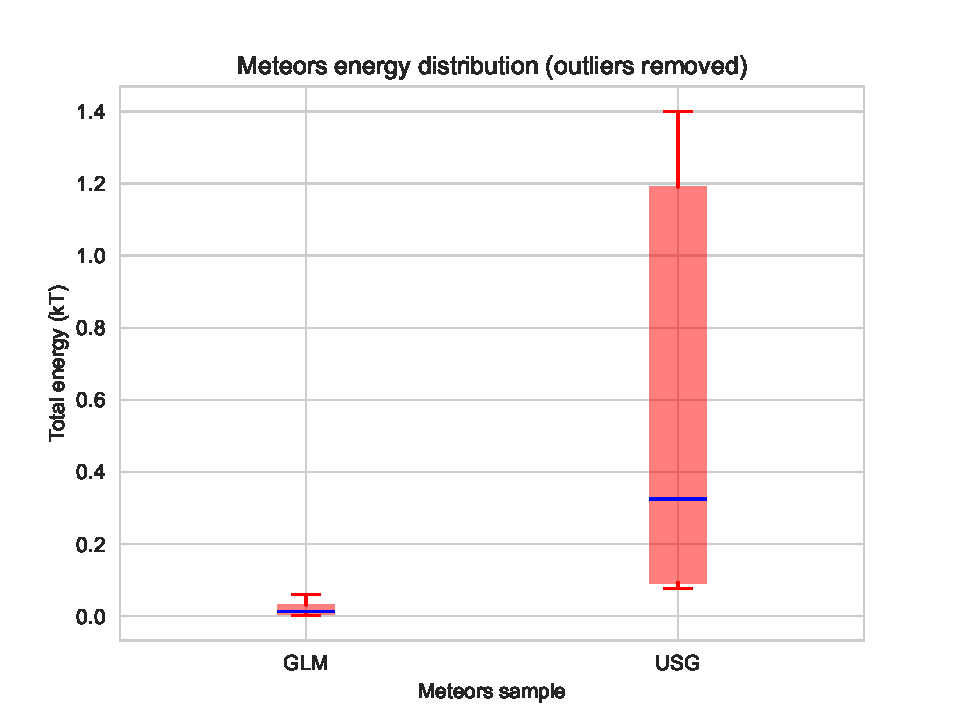
\includegraphics[width=\linewidth]{./figures/energies_boxplot}
  \caption{Comparison between released energies of bolides detected by the Geostationary Lightning Mapper and USG sensors.}
  \label{fig:boxplot}
\end{figure}


\subsection{GPS data}
\label{ssec:GPS}
%This material is based on services provided by the GAGE Facility, operated by UNAVCO, Inc., with support from the National Science Foundation and the National Aeronautics and Space Administration under NSF Cooperative Agreement EAR-1724794.

%We got RINEX data from 3 to 7 stations depending of the event location and data availability that surround the event place in all directions as possible. A list of the stations where we got RINEX data is available in table \ref{tab:table-stations}. Most of the stations lie in mexican territory, but in some cases we required data from other stations to cover events near the mexican frontier at north or south.

%\clearpage
%\onecolumn
%\footnotesize
%\begin{landscape}
%%\begin{table*}
%%    \centering
%  \begin{longtable}{llllllp{12cm}}
%      \caption{List of GPS stations used for this work.}
%      \label{tab:table-stations}
%      \endfirsthead
%      \endhead
%    \hline
%    Station name & Latitude & Longitude & \multicolumn{3}{c}{Events ID}  & Citation \\\hline
%    \multirow{4}{*}{BAR1\hyperlink{Hudnut}{${}^1$}\hyperlink{Hudnut2}{${}^5$}} & \multirow{4}{*}{33.48} & \multirow{4}{*}{-119.03} & \multirow{4}{*}{GLM-07} & \multirow{4}{*}{GLM-12} & \multirow{4}{*}{GLM-13} & UNAVCO Community, Hudnut, Kenneth, King, Nancy, Aspiotes, Aris G., Borsa, Adrian A., Determan, \\
%    &&&&&& Daniel N., Galetzka, John E., Stark, Keith F., 2005, SCIGN-PBO Nucleus GPS Network - BAR1-Santa \\
%    &&&&&& Barbara Island One P.S., The GAGE Facility operated by UNAVCO, Inc., GPS/GNSS Observations Dataset, \\
%    &&&&&& \url{https://doi.org/10.7283/T5668BHN}.\\\hline
%    \multirow{3}{*}{BLYT\hyperlink{Hudnut}{${}^1$}} & \multirow{3}{*}{33.61} & \multirow{3}{*}{-114.71} &  \multirow{3}{*}{GLM-12} & \multirow{3}{*}{GLM-13}  & & Hudnut, Kenneth, King, Nancy, Aspiotes, Aris G., Borsa, Adrian A., Determan, Daniel N., Galetzka, John \\
%    &&&&&& E., Stark, Keith F., 2006, SCIGN USGS GPS Network - BLYT-Blythe P.S., The GAGE Facility operated \\
%    &&&&&&  by UNAVCO, Inc., GPS/GNSS Observations Dataset, \url{https://doi.org/10.7283/T5HT2MKK}.\\\hline
%    \multirow{3}{*}{CN23} & \multirow{3}{*}{17.26} & \multirow{3}{*}{-88.78} &\multirow{3}{*}{GLM-08} & \multirow{3}{*}{GLM-15} & \multirow{3}{*}{GLM-16} & UNAVCO Community, 2012, COCONet GPS Network - CN23-BelmopanBZCR2012 P.S., The GAGE \\
%    &&&&&& Facility operated by UNAVCO, Inc., GPS/GNSS Observations Dataset, \\
%    &&&&&& \url{https://doi.org/10.7283/T5Q23XJH}.\\\hline
%    \multirow{3}{*}{CN25} & \multirow{3}{*}{16.23} & \multirow{3}{*}{-92.13} & \multirow{3}{*}{GLM-15} & & & UNAVCO Community, 2014, COCONet GPS Network - CN25-ComitandDMEX2012 P.S., The GAGE Facility operated by UNAVCO, Inc., GPS/GNSS Observations Dataset, \url{https://doi.org/10.7283/T57W69G7}.\\\hline
%    \multirow{3}{*}{GCFS} & \multirow{3}{*}{19.31} & \multirow{3}{*}{-81.18} & \multirow{3}{*}{GLM-08} & & & Watts, Anthony, 2016, COCONet GPS Network - GCFS-G\_CAYMAN\_CYM2014 P.S., The GAGE Facility operated by UNAVCO, Inc., GPS/GNSS Observations Dataset, \url{https://doi.org/10.7283/7ETV-X536}.\\\hline
%    \multirow{4}{*}{GMPK\hyperlink{Hudnut}{${}^1$}} & \multirow{4}{*}{33.05} & \multirow{4}{*}{-114.83} & \multirow{4}{*}{GLM-10} & & & UNAVCO Community, Hudnut, Kenneth, King, Nancy, Aspiotes, Aris G., Borsa, Adrian A., Determan, \\
%    &&&&&& Daniel N., Galetzka, John E., Stark, Keith F., 2005, SCIGN-PBO Nucleus GPS Network - GMPK-Glamis \\
%    &&&&&& Peak P.S., The GAGE Facility operated by UNAVCO, Inc., GPS/GNSS Observations Dataset, \\
%    &&&&&& \url{https://doi.org/10.7283/WCHN-H687}.\\\hline
%    \multirow{3}{*}{GUAT\hyperlink{Garnier}{${}^2$}} & \multirow{3}{*}{14.59} & \multirow{3}{*}{-90.52} & \multirow{3}{*}{GLM-16} & & & DeMets, Charles, Cosenza-Muralles, Beatriz, 2021, Central America 2018 - Guatemala, The GAGE \\
%    &&&&&& Facility operated by UNAVCO, Inc., GPS/GNSS Observations Dataset, \\
%    &&&&&& \url{https://doi.org/10.7283/KH2R-K704}.\\\hline
%\multirow{4}{*}{GUAX\hyperlink{Hudnut}{${}^1$}} & \multirow{4}{*}{28.88} & \multirow{4}{*}{-118.29} & GLM-05 & GLM-07 & GLM-11 & Hudnut, Kenneth, King, Nancy, Aspiotes, Aris G., Borsa, Adrian A., Determan, Daniel N., Galetzka, John \\
%    &&&GLM-12& GLM-13& GLM-18 & E., Stark, Keith F., 2001, SCIGN USGS GPS Network - GUAX-Isla Guadalupe P.S., The GAGE Facility \\
%    &&& GLM-25 &GLM-27 &GLM-28& operated by UNAVCO, Inc., GPS/GNSS Observations Dataset, \url{https://doi.org/10.7283/T5GX48T2}.\\
%    &&& GLM-32 &       &     &  \\\hline
%    \multirow{3}{*}{IAGX} & \multirow{3}{*}{29.03} & \multirow{3}{*}{-113.17} & \multirow{3}{*}{GLM-10} & & & Gonzalez-Ortega, Alejandro, Galetzka, John E., Gonzalez, Javier, 2018, CICESE REGNOM GPS Network \\
%    &&&&&& - IAGX-iagxREGNOMmx2018 P.S., The GAGE Facility operated by UNAVCO, Inc., GPS/GNSS  \\
%    &&&&&& Observations Dataset, \url{https://doi.org/10.7283/DGWN-A627}. \\\hline
%    \multirow{2}{*}{INEG} & \multirow{2}{*}{21.85} & \multirow{2}{*}{-102.28} & GLM-25 & GLM-26 & GLM-28  & No citations were found \\
%    &&& GLM-29 & GLM-30 & GLM-31 & \\\hline 
%    \multirow{4}{*}{KVTX} & \multirow{4}{*}{27.55} & \multirow{4}{*}{-97.89} & GLM-01 & GLM-02 & GLM-03  & UNAVCO Community, 2007, PBO GPS Network - KVTX-KingsvilleTX2006 P.S., The GAGE Facility \\
%    &&& GLM-04 & GLM-06 & GLM-19 & operated by UNAVCO, Inc., GPS/GNSS Observations Dataset, \url{https://doi.org/10.7283/T5J38QH8}.\\
%    &&& GLM-20 & GLM-21 & GLM-24 & \\
%    &&& GLM-26 &&& \\\hline
%    MDO1 & 30.68 & -104.02 & GLM-02 & & & No citations were found\\\hline
%    MGO5 & 30.68 & -104.02 & GLM-21 &GLM-26 &  & No citations were found\\\hline
%    MGW3 & 29.62 & -89.95 & GLM-19 & GLM-21 & GLM-24 & No citations were found\\\hline
%    \multirow{3}{*}{OXTH} & \multirow{3}{*}{16.29} & \multirow{3}{*}{-95.24} & \multirow{3}{*}{GLM-15} & \multirow{3}{*}{GLM-16} & & DeMets, Charles, Cabral-Cano, Enrique, 2008, Oaxaca GPS Network - OXTH-Tehuantepec P.S., The \\
%    &&&&&& GAGE Facility operated by UNAVCO, Inc., GPS/GNSS Observations Dataset, \\
%    &&&&&& \url{https://doi.org/10.7283/T5Q81B5V}.\\\hline
%    \multirow{3}{*}{OXUM\hyperlink{Graham}{${}^3$}} & \multirow{3}{*}{15.66} & \multirow{3}{*}{-96.50} & \multirow{3}{*}{GLM-34} & & & Cabral-Cano, Enrique, Salazar-Tlaczani, Luis, 2015, TLALOCNet - OXUM-oxum\_tnet\_mx2001 P.S., The \\
%    &&&&&& GAGE Facility operated by UNAVCO, Inc., GPS/GNSS Observations Dataset, \\
%    &&&&&& \url{https://doi.org/10.7283/T5J964RP}.\\\hline
%    \multirow{2}{*}{P001} & \multirow{2}{*}{31.95} & \multirow{2}{*}{-112.80} & \multirow{2}{*}{GLM-07} & \multirow{2}{*}{GLM-22} & & UNAVCO Community, 2008, PBO GPS Network - P001-Organ\_PipeAZ2007 P.S., The GAGE Facility \\
%    &&&&&& operated by UNAVCO, Inc., GPS/GNSS Observations Dataset, \url{https://doi.org/10.7283/T5DR2SGP}.\\\hline
%    \multirow{2}{*}{P014} & \multirow{2}{*}{31.97} & \multirow{2}{*}{-11.09} & GLM-10 & GLM-12 & GLM-13 & UNAVCO Community, 2008, PBO GPS Network - P014-Sahuarita\_AZ2007 P.S., The GAGE Facility \\
%    &&& GLM-14 & GLM-22 & & operated by UNAVCO, Inc., GPS/GNSS Observations Dataset, \url{https://doi.org/10.7283/T5DJ5CMK}.\\\hline
%    \multirow{2}{*}{P807} & \multirow{2}{*}{30.49} & \multirow{2}{*}{-98.82} & GLM-06 & GLM-14 & GLM-21 & UNAVCO Community, 2012, PBO GPS Network - P807-EcRockStPkTX2012 P.S., The GAGE Facility \\
%    &&& GLM-30 &&& operated by UNAVCO, Inc., GPS/GNSS Observations Dataset, \url{https://doi.org/10.7283/T5TQ5ZKM}.\\\hline
%    \multirow{2}{*}{PLPX} & \multirow{2}{*}{31.59} & \multirow{2}{*}{-115.15} & \multirow{2}{*}{GLM-10} & & & UNAVCO Community, 2011, PBO GPS Network - PLPX-Las\_PintasMX2010 P.S., The GAGE Facility \\
%    &&&&&& operated by UNAVCO, Inc., GPS/GNSS Observations Dataset, \url{https://doi.org/10.7283/T5K64G3T}.\\\hline
%    \multirow{2}{*}{PTEX} & \multirow{2}{*}{32.29} & \multirow{2}{*}{-116.52} & GLM-07 & GLM-12 & GLM-13  & UNAVCO Community, 2011, PBO GPS Network - PTEX-Testerazo\_MX2011 P.S., The GAGE Facility \\
%    &&& GLM-27 & GLM-32 & & operated by UNAVCO, Inc., GPS/GNSS Observations Dataset, \url{https://doi.org/10.7283/T5610XBP}.\\\hline 
%    \multirow{3}{*}{RG06} & \multirow{3}{*}{32.63} & \multirow{3}{*}{-107.86} & \multirow{3}{*}{GLM-22} & & & Sheehan, Anne, 2007, Rio Grande Rift GPS Network - RG06-RG06FaywodNM2006 P.S., The GAGE \\
%    &&&&&& Facility operated by UNAVCO, Inc., GPS/GNSS Observations Dataset, \\
%    &&&&&& \url{https://doi.org/10.7283/T5668BFR}.\\\hline
%    \multirow{3}{*}{RG07} & \multirow{3}{*}{32.50} & \multirow{3}{*}{-106.84} & \multirow{3}{*}{GLM-14} & & & Sheehan, Anne, 2007, Rio Grande Rift GPS Network - RG07-RG07CrucesNM2006 P.S., The GAGE  \\
%    &&&&&& Facility operated by UNAVCO, Inc., GPS/GNSS Observations Dataset, \\
%    &&&&&& \url{https://doi.org/10.7283/T5KD1W45}. \\\hline
%    \multirow{3}{*}{SG33} & \multirow{3}{*}{31.77} & \multirow{3}{*}{-106.51} & \multirow{3}{*}{GLM-06} & \multirow{3}{*}{GLM-20} & \multirow{3}{*}{GLM-26} & Harder, Steven, Kaip, Galen, Montana, Carlos, 2004, SuomiNet-G GPS Network - SG33-UTEP P.S., The \\
%    &&&&&& GAGE Facility operated by UNAVCO, Inc., GPS/GNSS Observations Dataset,  \\
%    &&&&&& \url{https://doi.org/10.7283/T50863KQ}. \\\hline
%    \multirow{3}{*}{TGMX}  & \multirow{3}{*}{20.87} & \multirow{3}{*}{-86.87} & \multirow{3}{*}{GLM-34} & & & UNAVCO Community, 2015, COCONet GPS Network - TGMX-PtoMor\_TG\_MX2015 P.S., The GAGE \\
%    &&&&&& Facility operated by UNAVCO, Inc., GPS/GNSS Observations Dataset,  \\
%    &&&&&& \url{https://doi.org/10.7283/T5154FB7}. \\\hline
%    \multirow{2}{*}{TNAM} & \multirow{2}{*}{20.54} & \multirow{2}{*}{-103.97} & GLM-17 & GLM-25 & GLM-28  & UNAVCO Community, 2014, TLALOCNet - TNAM-TNAM\_TNET\_MX2014 P.S., The GAGE Facility \\
%    &&& GLM-29 & GLM-30 & GLM-31 & operated by UNAVCO, Inc., GPS/GNSS Observations Dataset, \url{https://doi.org/10.7283/T5QF8R4R}.\\\hline
%    \multirow{2}{*}{TNAT} & \multirow{2}{*}{18.13} & \multirow{2}{*}{-98.04} & \multirow{2}{*}{GLM-15} & & & UNAVCO Community, 2014, TLALOCNet - TNAT-TNAT\_TNET\_MX2014 P.S., The GAGE Facility \\
%    &&&&&& operated by UNAVCO, Inc., GPS/GNSS Observations Dataset, \url{https://doi.org/10.7283/T5G15Z4S}. \\\hline
%    \multirow{2}{*}{TNBA} & \multirow{2}{*}{28.97} & \multirow{2}{*}{-113.55} & GLM-05 & GLM-07 & GLM-09  & UNAVCO Community, 2015, TLALOCNet - TNBA-TNBA\_TNET\_MX2014 P.S., The GAGE Facility  \\
%    &&& GLM-11 & GLM-12 & GLM-13 & operated by UNAVCO, Inc., GPS/GNSS Observations Dataset, \url{https://doi.org/10.7283/T57M0688}.\\\hline
%    \multirow{2}{*}{TNCC} & \multirow{2}{*}{18.79} & \multirow{2}{*}{-103.17} & \multirow{2}{*}{GLM-17} & & & UNAVCO Community, 2015, TLALOCNet - TNCC-TNCC\_TNET\_MX2015 P.S., The GAGE Facility \\
%    &&&&&& operated by UNAVCO, Inc., GPS/GNSS Observations Dataset, \url{https://doi.org/10.7283/T50R9MSK}.\\\hline
%    \multirow{2}{*}{TNCM} & \multirow{2}{*}{19.50} & \multirow{2}{*}{-105.04} & \multirow{2}{*}{GLM-17} & \multirow{2}{*}{GLM-23} & & UNAVCO Community, 2014, TLALOCNet - TNCM-TNCM\_TNET\_MX2014 P.S., The GAGE Facility \\
%    &&&&&& operated by UNAVCO, Inc., GPS/GNSS Observations Dataset, \url{https://doi.org/10.7283/T5B856FW}.\\\hline
%    \multirow{2}{*}{TNCN} & \multirow{2}{*}{18.55} & \multirow{2}{*}{-101.97} & \multirow{2}{*}{GLM-29} & \multirow{2}{*}{GLM-33} & & UNAVCO Community, 2016, TLALOCNet - TNCN-TNCN\_TNET\_MX2016 P.S., The GAGE Facility \\
%    &&&&&& operated by UNAVCO, Inc., GPS/GNSS Observations Dataset, \url{https://doi.org/10.7283/T5610XQM}.\\\hline
%    \multirow{4}{*}{TNCU} & \multirow{4}{*}{28.45} & \multirow{4}{*}{-106.79} & GLM-01 & GLM-02 & GLM-03  & UNAVCO Community, 2014, TLALOCNet - TNCU-CuauhtemocTN2014 P.S., The GAGE Facility \\
%    &&& GLM-06 & GLM-11 & GLM-14 & operated by UNAVCO, Inc., GPS/GNSS Observations Dataset, \url{https://doi.org/10.7283/T5V69GV2}.\\
%    &&& GLM-18 & GLM-20 & GLM-25 & \\
%    &&& GLM-26 & GLM-30 & GLM-31 & \\\hline
%    \multirow{3}{*}{TNGF} & \multirow{3}{*}{19.33} & \multirow{3}{*}{-99.18} & \multirow{3}{*}{GLM-29} & \multirow{3}{*}{GLM-33} & & Cabral-Cano, Enrique, Salazar-Tlaczani, Luis, 2016, TLALOCNet GPS Network - TNGF\_Geofisica-\\
%    &&&&&& UNAM\_Mexico\_City\_TNET\_mx2015 P.S., The GAGE Facility operated by UNAVCO, Inc., GPS/GNSS \\
%    &&&&&& Observations Dataset, \url{https://doi.org/10.7283/T53X851M}. \\\hline
%    \multirow{5}{*}{TNHM} & \multirow{5}{*}{29.08} & \multirow{5}{*}{-110.97} & GLM-05 & GLM-09 & GLM-10 & UNAVCO Community, 2014, TLALOCNet - TNHM-hermosilloTN2014 P.S., The GAGE Facility \\
%    &&& GLM-11 & GLM-12 & GLM-13 & operated by UNAVCO, Inc., GPS/GNSS Observations Dataset, \url{https://doi.org/10.7283/T5KP80FV}.\\
%    &&& GLM-18 & GLM-20 & GLM-25 & \\
%    &&& GLM-26 & GLM-27 & GLM-28 & \\
%    &&& GLM-32 &        &        & \\\hline
%    \multirow{2}{*}{TNMS} & \multirow{2}{*}{20.53} & \multirow{2}{*}{-104.80} & GLM-05 & GLM-09 & GLM-11  & UNAVCO Community, 2014, TLALOCNet - TNMS-TNMS\_TNET\_MX2014 P.S., The GAGE Facility \\
%    &&& GLM-17 & GLM-25 & & operated by UNAVCO, Inc., GPS/GNSS Observations Dataset, \url{https://doi.org/10.7283/T56H4FQ5}.\\\hline
%    \multirow{3}{*}{TNNP} & \multirow{3}{*}{16.12} & \multirow{3}{*}{-97.14} & \multirow{3}{*}{GLM-23} & & & Cabral-Cano, Enrique, Salazar-Tlaczani, Luis, DeMets, Charles, 2016, TLALOCNet - TNNP-\\
%    &&&&&& tnnp\_tnet\_mx2015 P.S., The GAGE Facility operated by UNAVCO, Inc., GPS/GNSS Observations Dataset, \\
%    &&&&&& \url{https://doi.org/10.7283/T5N29V96}. \\\hline
%    \multirow{2}{*}{TNNX} & \multirow{2}{*}{17.41} & \multirow{2}{*}{-97.22} & GLM-15 & GLM-16 & GLM-33  & UNAVCO Community, 2014, TLALOCNet - TNNX-TNNX\_TNET\_MX2014 P.S., The GAGE Facility \\
%    &&& GLM-34 &&& operated by UNAVCO, Inc., GPS/GNSS Observations Dataset, \url{https://doi.org/10.7283/T52R3PZ0}.\\\hline
%    \multirow{2}{*}{TNPP} & \multirow{2}{*}{31.34} & \multirow{2}{*}{-113.63} & GLM-07 & GLM-10 & GLM-18 & UNAVCO Community, 2015, TLALOCNet - TNPP-TNPP\_TNET\_MX2015 P.S., The GAGE Facility \\
%    &&& GLM-22 &&& operated by UNAVCO, Inc., GPS/GNSS Observations Dataset, \url{https://doi.org/10.7283/T5CC0Z0M}.\\\hline
%    \multirow{2}{*}{TNSJ} & \multirow{2}{*}{16.17} & \multirow{2}{*}{-96.49} & \multirow{2}{*}{GLM-33} & & & UNAVCO Community, 2016, TLALOCNet - TNSJ-tnsj\_tnet\_mx2015 P.S., The GAGE Facility operated by \\
%    &&&&&& UNAVCO, Inc., GPS/GNSS Observations Dataset, \url{https://doi.org/10.7283/T59S1PF1}.\\\hline
%    \multirow{3}{*}{TSFX} & \multirow{3}{*}{30.93} & \multirow{3}{*}{-114.81} & \multirow{3}{*}{GLM-07} & \multirow{3}{*}{GLM-27} & \multirow{3}{*}{GLM-32} & Gonzalez-Ortega, Alejandro, Galetzka, John E., Gonzalez, Javier, 2018, CICESE REGNOM GPS Network \\
%    &&&&&& - TSFX-tsfxREGNOMmx2016 P.S., The GAGE Facility operated by UNAVCO, Inc., GPS/GNSS \\
%    &&&&&& Observations Dataset, \url{https://doi.org/10.7283/AGEA-2G27}.\\\hline
%    \multirow{3}{*}{UAGU} & \multirow{3}{*}{21.92} & \multirow{3}{*}{-102.32} & GLM-01 & GLM-02 & GLM-03  & Cabral-Cano, Enrique, Salazar-Tlaczani, Luis, 2015, TLALOCNet - UAGU-uagu\_tnet\_mx2008 P.S., The \\
%    &&& GLM-04 & GLM-06 & GLM-09 & GAGE Facility operated by UNAVCO, Inc., GPS/GNSS Observations Dataset, \\
%    &&& GLM-11 & GLM-20 &        & \url{https://doi.org/10.7283/T5513WK7}.\\\hline
%    \multirow{3}{*}{UCOE\hyperlink{Graham}{${}^3$}} & \multirow{3}{*}{19.81} & \multirow{3}{*}{-101.69} & GLM-03 & GLM-06 & GLM-30 & Cabral-Cano, Enrique, Salazar-Tlaczani, Luis, 2015, TLALOCNet - UCOE-ucoe\_tnet\_mx2003 P.S., The \\
%    &&& GLM-31 &&& GAGE Facility operated by UNAVCO, Inc., GPS/GNSS Observations Dataset, \\
%    &&&&&& \url{https://doi.org/10.7283/T51834VW}. \\\hline
%    \multirow{3}{*}{UGEO\hyperlink{Marquez}{${}^4$}} & \multirow{3}{*}{20.69} & \multirow{3}{*}{-103.35} & \multirow{3}{*}{GLM-03} & & & Marquez-Azua, Bertha, DeMets, Charles, Cabral-Cano, Enrique, Salazar-Tlaczani, Luis, 2015, \\
%    &&&&&& TLALOCNet - UGEO-ugeo\_tnet\_mx1998 P.S., The GAGE Facility operated by UNAVCO, Inc., GPS/GNSS \\
%    &&&&&& Observations Dataset, \url{https://doi.org/10.7283/T58S4N9N}. \\\hline
%    \multirow{2}{*}{UHSL} & \multirow{2}{*}{29.57} & \multirow{2}{*}{-95.65} & \multirow{2}{*}{GLM-19} & & & Wang, Guoquan, 2014, HoustonNet GPS Network - UHSL-SugarLandUSA2014 P.S., The GAGE Facility \\
%    &&&&&& operated by UNAVCO, Inc., GPS/GNSS Observations Dataset, \url{https://doi.org/10.7283/T55X271S}.\\\hline
%    \multirow{3}{*}{UHWL} & \multirow{3}{*}{30.06} & \multirow{3}{*}{-94.98} & \multirow{3}{*}{GLM-31} & & & Wang, Guoquan, 2014, HoustonNet GPS Network - UHWL-West Liberty Airport(Deep) P.S., The GAGE \\
%    &&&&&& Facility operated by UNAVCO, Inc., GPS/GNSS Observations Dataset,  \\
%    &&&&&& \url{https://doi.org/10.7283/T53R0R5P}. \\\hline
%    \multirow{3}{*}{UNPM} & \multirow{3}{*}{20.86} & \multirow{3}{*}{-86.86} & GLM-08 & GLM-15 & GLM-16  & UNAVCO Community, 2012, COCONet GPS Network - UNPM-Puerto\_Morelos\_MX\_2007 P.S., The \\
%    &&& GLM-24 &&& GAGE Facility operated by UNAVCO, Inc., GPS/GNSS Observations Dataset, \\
%    &&&&&& \url{https://doi.org/10.7283/J1GD-5S40}.\\\hline
%    \multirow{3}{*}{USMX} & \multirow{3}{*}{29.82} & \multirow{3}{*}{-109.68} & GLM-12 & GLM-13 & GLM-14  & Bennett, Rick, 2004, Northwest Mexico GPS Network - USMX-Universidad de la Sierra P.S., The GAGE \\
%    &&& GLM-22 & GLM-26 & GLM-28 & Facility operated by UNAVCO, Inc., GPS/GNSS Observations Dataset, \\
%    &&&&&& \url{https://doi.org/10.7283/T5W957CQ}.\\\hline
%    \multirow{3}{*}{UXAL\hyperlink{Graham}{${}^3$}} & \multirow{3}{*}{19.52} & \multirow{3}{*}{-96.92} & GLM-04 & GLM-15 & GLM-16  & Cabral-Cano, Enrique, Salazar-Tlaczani, Luis, 2015, TLALOCNet - UXAL-uxal\_tnet\_mx2005 P.S., The \\
%    &&& GLM-19 & GLM-24 & GLM-31 & GAGE Facility operated by UNAVCO, Inc., GPS/GNSS Observations Dataset, \\
%    &&& GLM-34 &        &        & \url{https://doi.org/10.7283/T5DJ5D1C}.\\\hline
%    \multirow{2}{*}{WEPD} & \multirow{2}{*}{29.69} & \multirow{2}{*}{-95.23} & \multirow{2}{*}{GLM-21} & & & Wang, Guoquan, 2014, HoustonNet GPS Network - WEPD-willmselementary P.S., The GAGE Facility \\
%    &&&&&& operated by UNAVCO, Inc., GPS/GNSS Observations Dataset, \url{https://doi.org/10.7283/T5NZ85RB}. \\\hline
%    \multirow{2}{*}{WMOK} & \multirow{2}{*}{34.74} & \multirow{2}{*}{-98.78} & \multirow{2}{*}{GLM-21} & & & UNAVCO Community, 2005, PBO GPS Network - WMOK-WichitaMtnOK2005 P.S., The GAGE Facility \\
%    &&&&&& operated by UNAVCO, Inc., GPS/GNSS Observations Dataset, \url{https://doi.org/10.7283/T59021Q6}. \\\hline
%    \multirow{4}{*}{WWMT\hyperlink{Hudnut}{${}^1$}} & \multirow{4}{*}{33.96} & \multirow{4}{*}{-116.65} & \multirow{4}{*}{GLM-07} & \multirow{4}{*}{GLM-12} & \multirow{4}{*}{GLM-13} & Hudnut, Kenneth, King, Nancy, Aspiotes, Aris G., Borsa, Adrian A., Determan, Daniel N., Galetzka, John \\
%    &&&&&& E., Stark, Keith F., 2006, SCIGN USGS GPS Network - WWMT-Whitewater Mountain P.S., The GAGE \\
%    &&&&&& Facility operated by UNAVCO, Inc., GPS/GNSS Observations Dataset,  \\
%    &&&&&& \url{https://doi.org/10.7283/T5H993F2}. \\\hline
%    \multirow{2}{*}{YESX} & \multirow{2}{*}{28.38} & \multirow{2}{*}{-108.92} & GLM-09 & GLM-11 & GLM-14  & Bennett, Rick, 2004, Northwest Mexico GPS Network - YESX-Yecora P.S., The GAGE Facility operated \\
%    &&&GLM-20 & GLM-23 & GLM-25 & by UNAVCO, Inc., GPS/GNSS Observations Dataset, \url{https://doi.org/10.7283/T5RJ4GPF}.\\\hline
%    
%%    % \end{table*}
%  \end{longtable}
%    \begin{minipage}{0.9\linewidth}
%      \footnotesize
%      Related articles:
%      
%      \hypertarget{Hudnut}{${}^1$}\citet{Hudnut:2002},
%      %
%      \hypertarget{Garnier}{${}^2$}\citet{Garnier:2021}, 
%      %
%      \hypertarget{Graham}{${}^3$}\citet{Graham:2016}
%      
%      \hypertarget{Marquez}{${}^4$}\href{https://doi.org/10.7283/T58S4N9N}{B. Marquez-Azua, E. Cabral-Cano, F. Correa-Mora and C. DeMets, 2004. A model for Mexican neotectonics based on Nationwide GPS measurements, 1993-2001, Geofisica Internacional, v. 43, p.319-330}
%      
%      \hypertarget{Hudnut2}{${}^5$}\href{https://doi.org/10.7283/T5668BHN}{Hudnut, K. W., Y. Bock, J. E. Galetzka, F. H. Webb, and W. H. Young, The Southern California Integrated GPS Network (SCIGN), Proceedings of the International Workshop on Seismotectonics at the Subduction Zone, Y. Fujinawa (ed.), NIED, Tsukuba, Japan, pp. 175-196, 1999}    
%    \end{minipage}
%  \end{landscape}
%  \clearpage
%  \twocolumn

%  The obtained RINEX files are compressed in Hatanaka format, developed at the Geographical Survey Institute by Y. Hatanaka \citep{Kumar:2012}. From this files we may estimate the Slant Total Electron Content (sTEC) and the Vertical Total Electron Content (vTEC) which may be computed in the following way:

  The Total Electron content along the integrated path of the link $(s_i)$ at the frequency $f_i$ can be inferred from the phase delay $L_i$ of the frequency $f_i$ \citep{Emery:2017}:
  \begin{align}
    L_i = s_i - \frac{\SI{40.3082}{m^3.s^{-1}}}{f_i^2}sTEC_i
  \end{align}
  Combining two observations at two different frequencies $f_1$ and $f_2$ we may obtain two different phase delays $L_1$ and $L_2$ and derive the TEC along the signal path:

  \begin{align}
    sTEC = \frac{f_1^2f_2^2\left(L_1-L_2\right)}{\SI{40.3082}{m^3.s^{-1}}\left(f_1^2-f_2^2\right)}
  \end{align}

  In the other hand, the Vertical Total Electron Content (vTEC) is computed from the sTEC as follows \citep{Kumar:2012}:
  \begin{align}
    vTEC = \frac{sTEC-\left[b_R+b_S\right]}{S(\theta_I)}
  \end{align}

  where $b_R$ and $b_S$ are receiver and satellite biases, respectively. $\theta_I$ is the elevation angle in degrees, $S(\theta_I)$ is the obliquity factor with zenith angle $\psi$ at the Ionospheric Pierce Point (IPP):

  \begin{align}
    S(\theta_i) = \frac{1}{\cos\psi} = \left\lbrace 1-\frac{R_E\cos\theta_I}{R_E+h}\right\rbrace^{-1/2}
  \end{align}

  Where $R_E$ is the Earth radius in km and $h=\SI{350}{km}$ is the ionospheric shell above the earth's surface.

  Both parameters sTEC and vTEC are computed using a software developed by Gopi K. Seemala, publicly available at \url{https://seemala.blogspot.com/}.

  
%For the selected sample, we obtained RINEX data from the TlalocNet \citep{Cabral-Cano:2018} and UNAVCO network databases to study potential alterations in the ionospehre due to the presence of the passing meteor at the day the meteor was reported. For each event, we downloaded data from stations that surrounds the place where the event was detected (usually 3 to 5 stations. )The list of the sample meteors is shown in table \ref{tab:table-meteors}. The events are in chronological order. The reported duration, latitude and longitude correspond to the mean between measurements from satellites GOES-16 and GOES 17; in the same way, the uncertainties correspond to the standard deviation. Also their respective positions are available in figure \ref{fig:meteors-map}, where each label correspond to the ID (first column) of table \ref{tab:table-meteors}.
     
%Using the data provided by TlalocNet and UNAVCO, we procceeded to obtain TEC parameters with the GPS\_GOPI software, available at \url{https://seemala.blogspot.com/}. This software takes as input the RINEX data (the navigation file is no strictly neccesary), and the outuput consists in in the vTEC and sTEC measurements for the PRNs of the whole day the event occurred, as well as the averaged TEC as function of time. We obtained vTEC maps for the events in table (\ref{tab:table-meteors}) and their respective next and previous day.
     
%Final idea: use GOPI software to get the vTEC data from the day of each event and the previous days.

%Materials and Methods should be described with sufficient details to allow others to replicate and build on published results. Please note that publication of your manuscript implicates that you must make all materials, data, computer code, and protocols associated with the publication available to readers. Please disclose at the submission stage any restrictions on the availability of materials or information. New methods and protocols should be described in detail while well-established methods can be briefly described and appropriately cited.

%Research manuscripts reporting large datasets that are deposited in a publicly avail-able database should specify where the data have been deposited and provide the relevant accession numbers. If the accession numbers have not yet been obtained at the time of submission, please state that they will be provided during review. They must be provided prior to publication.

%Interventionary studies involving animals or humans, and other studies require ethical approval must list the authority that provided approval and the corresponding ethical approval code.
%\begin{quote}
%This is an example of a quote.
%\end{quote}

%%%%%%%%%%%%%%%%%%%%%%%%%%%%%%%%%%%%%%%%%%
\section{Results}

%This section may be divided by subheadings. It should provide a concise and precise description of the experimental results, their interpretation as well as the experimental conclusions that can be drawn.
%\%subsection{Subsection}
%\subsubsection{Subsubsection}

%Bulleted lists look like this:
%\begin{itemize}
%\item	First bullet;
%\item	Second bullet;
%\item	Third bullet.
%\end{itemize}

%Numbered lists can be added as follows:
%\begin{enumerate}
%\item	First item; 
%\item	Second item;
%\item	Third item.
%\end{enumerate}

%The text continues here. 

%\subsection{Figures, Tables and Schemes}

%All figures and tables should be cited in the main text as Figure~\ref{fig1}, Table~\ref{tab1}, Table~\ref{tab2}, etc.

%\begin{figure}[H]
%\includegraphics[width=10.5 cm]{Definitions/logo-mdpi}
%\caption{This is a figure. Schemes follow the same formatting. If there are multiple panels, they should be listed as: (\textbf{a}) Description of what is contained in the first panel. (\textbf{b}) Description of what is contained in the second panel. Figures should be placed in the main text near to the first time they are cited. A caption on a single line should be centered.\label{fig1}}
%\end{figure}   
%\unskip

%\begin{table}[H] 
%\caption{This is a table caption. Tables should be placed in the main text near to the first time they are~cited.\label{tab1}}
%\newcolumntype{C}{>{\centering\arraybackslash}X}
%\begin{tabularx}{\textwidth}{CCC}
%\toprule
%\textbf{Title 1}	& \textbf{Title 2}	& \textbf{Title 3}\\
%\midrule
%Entry 1		& Data			& Data\\
%Entry 2		& Data			& Data\\
%\bottomrule
%\end{tabularx}
%\end{table}
%\unskip

%\begin{table}[H]
%\caption{This is a wide table.\label{tab2}}
%	\begin{adjustwidth}{-\extralength}{0cm}
%		\newcolumntype{C}{>{\centering\arraybackslash}X}
%		\begin{tabularx}{\textwidth+\extralength}{CCCC}
%			\toprule
%			\textbf{Title 1}	& \textbf{Title 2}	& \textbf{Title 3}     & \textbf{Title 4}\\
%			\midrule
%			Entry 1		& Data			& Data			& Data\\
%			Entry 2		& Data			& Data			& Data\textsuperscript{1}\\
%			\bottomrule
%		\end{tabularx}
%	\end{adjustwidth}
%	\noindent{\footnotesize{\textsuperscript{1} This is a table footnote.}}
%\end{table}

%\begin{listing}[H]
%\caption{Title of the listing}
%\rule{\columnwidth}{1pt}
%\raggedright Text of the listing. In font size footnotesize, small, or normalsize. Preferred format: left aligned and single spaced. Preferred border format: top border line and bottom border line.
%\rule{\columnwidth}{1pt}
%\end{listing}

%Text.

%Text.

%\subsection{Formatting of Mathematical Components}

%This is the example 1 of equation:
%\begin{linenomath}
%\begin{equation}
%a = 1,
%\end{equation}
%\end{linenomath}
%the text following an equation need not be a new paragraph. Please punctuate equations as regular text.
%% If the documentclass option "submit" is chosen, please insert a blank line before and after any math environment (equation and eqnarray environments). This ensures correct linenumbering. The blank line should be removed when the documentclass option is changed to "accept" because the text following an equation should not be a new paragraph.

%This is the example 2 of equation:
%\begin{adjustwidth}{-\extralength}{0cm}
%\begin{equation}
%a = b + c + d + e + f + g + h + i + j + k + l + m + n + o + p + q + r + s + t + u + v + w + x + y + z
%\end{equation}
%\end{adjustwidth}

% Example of a page in landscape format (with table and table footnote).
%\startlandscape
%\begin{table}[H] %% Table in wide page
%\caption{This is a very wide table.\label{tab3}}
%	\begin{tabularx}{\textwidth}{CCCC}
%		\toprule
%		\textbf{Title 1}	& \textbf{Title 2}	& \textbf{Title 3}	& \textbf{Title 4}\\
%		\midrule
%		Entry 1		& Data			& Data			& This cell has some longer content that runs over two lines.\\
%		Entry 2		& Data			& Data			& Data\textsuperscript{1}\\
%		\bottomrule
%	\end{tabularx}
%	\begin{adjustwidth}{+\extralength}{0cm}
%		\noindent\footnotesize{\textsuperscript{1} This is a table footnote.}
%	\end{adjustwidth}
%\end{table}
%\finishlandscape

% Example of a figure that spans the whole page width. The same concept works for tables, too.
%\begin{figure}[H]
%\begin{adjustwidth}{-\extralength}{0cm}
%\centering
%\includegraphics[width=15cm]{Definitions/logo-mdpi}
%\end{adjustwidth}
%\caption{This is a wide figure.\label{fig2}}
%\end{figure}  

%Please punctuate equations as regular text. Theorem-type environments (including propositions, lemmas, corollaries etc.) can be formatted as follows:
%% Example of a theorem:
%\begin{Theorem}
%Example text of a theorem.
%\end{Theorem}

%The text continues here. Proofs must be formatted as follows:

%% Example of a proof:
%\begin{proof}[Proof of Theorem 1]
%Text of the proof. Note that the phrase ``of Theorem 1'' is optional if it is clear which theorem is being referred to.
%\end{proof}
%The text continues here.

%%%%%%%%%%%%%%%%%%%%%%%%%%%%%%%%%%%%%%%%%%
%\section{Discussion}

%Authors should discuss the results and how they can be interpreted from the perspective of previous studies and of the working hypotheses. The findings and their implications should be discussed in the broadest context possible. Future research directions may also be highlighted.

%%%%%%%%%%%%%%%%%%%%%%%%%%%%%%%%%%%%%%%%%%
%\section{Conclusions}

This section is not mandatory, but can be added to the manuscript if the discussion is unusually long or complex.

%%%%%%%%%%%%%%%%%%%%%%%%%%%%%%%%%%%%%%%%%%
%\section{Patents}

%This section is not mandatory, but may be added if there are patents resulting from the work reported in this manuscript.

%%%%%%%%%%%%%%%%%%%%%%%%%%%%%%%%%%%%%%%%%%
\vspace{6pt} 

%%%%%%%%%%%%%%%%%%%%%%%%%%%%%%%%%%%%%%%%%%
%% optional
%\supplementary{The following are available online at \linksupplementary{s1}, Figure S1: title, Table S1: title, Video S1: title.}

% Only for the journal Methods and Protocols:
% If you wish to submit a video article, please do so with any other supplementary material.
% \supplementary{The following are available at \linksupplementary{s1}, Figure S1: title, Table S1: title, Video S1: title. A supporting video article is available at doi: link.} 

%%%%%%%%%%%%%%%%%%%%%%%%%%%%%%%%%%%%%%%%%%
\authorcontributions{For research articles with several authors, a short paragraph specifying their individual contributions must be provided. The following statements should be used ``Conceptualization, X.X. and Y.Y.; methodology, X.X.; software, X.X.; validation, X.X., Y.Y. and Z.Z.; formal analysis, X.X.; investigation, X.X.; resources, X.X.; data curation, X.X.; writing---original draft preparation, X.X.; writing---review and editing, X.X.; visualization, X.X.; supervision, X.X.; project administration, X.X.; funding acquisition, Y.Y. All authors have read and agreed to the published version of the manuscript.'', please turn to the  \href{http://img.mdpi.org/data/contributor-role-instruction.pdf}{CRediT taxonomy} for the term explanation. Authorship must be limited to those who have contributed substantially to the work~reported.}

\funding{Please add: ``This research received no external funding'' or ``This research was funded by NAME OF FUNDER grant number XXX.'' and  and ``The APC was funded by XXX''. Check carefully that the details given are accurate and use the standard spelling of funding agency names at \url{https://search.crossref.org/funding}, any errors may affect your future funding.}

\institutionalreview{In this section, please add the Institutional Review Board Statement and approval number for studies involving humans or animals. Please note that the Editorial Office might ask you for further information. Please add ``The study was conducted according to the guidelines of the Declaration of Helsinki, and approved by the Institutional Review Board (or Ethics Committee) of NAME OF INSTITUTE (protocol code XXX and date of approval).'' OR ``Ethical review and approval were waived for this study, due to REASON (please provide a detailed justification).'' OR ``Not applicable'' for studies not involving humans or animals. You might also choose to exclude this statement if the study did not involve humans or animals.}

\informedconsent{Any research article describing a study involving humans should contain this statement. Please add ``Informed consent was obtained from all subjects involved in the study.'' OR ``Patient consent was waived due to REASON (please provide a detailed justification).'' OR ``Not applicable'' for studies not involving humans. You might also choose to exclude this statement if the study did not involve humans.

Written informed consent for publication must be obtained from participating patients who can be identified (including by the patients themselves). Please state ``Written informed consent has been obtained from the patient(s) to publish this paper'' if applicable.}

\dataavailability{In this section, please provide details regarding where data supporting reported results can be found, including links to publicly archived datasets analyzed or generated during the study. Please refer to suggested Data Availability Statements in section ``MDPI Research Data Policies'' at \url{https://www.mdpi.com/ethics}. You might choose to exclude this statement if the study did not report any data.} 

\acknowledgments{In this section you can acknowledge any support given which is not covered by the author contribution or funding sections. This may include administrative and technical support, or donations in kind (e.g., materials used for experiments).}

\conflictsofinterest{Declare conflicts of interest or state ``The authors declare no conflict of interest.'' Authors must identify and declare any personal circumstances or interest that may be perceived as inappropriately influencing the representation or interpretation of reported research results. Any role of the funders in the design of the study; in the collection, analyses or interpretation of data; in the writing of the manuscript, or in the decision to publish the results must be declared in this section. If there is no role, please state ``The funders had no role in the design of the study; in the collection, analyses, or interpretation of data; in the writing of the manuscript, or in the decision to publish the~results''.} 

%% Optional
\sampleavailability{Samples of the compounds ... are available from the authors.}

%%%%%%%%%%%%%%%%%%%%%%%%%%%%%%%%%%%%%%%%%%
%% Only for journal Encyclopedia
%\entrylink{The Link to this entry published on the encyclopedia platform.}

%%%%%%%%%%%%%%%%%%%%%%%%%%%%%%%%%%%%%%%%%%
%% Optional
\abbreviations{Abbreviations}{
The following abbreviations are used in this manuscript:\\

\noindent 
\begin{tabular}{@{}ll}
MDPI & Multidisciplinary Digital Publishing Institute\\
DOAJ & Directory of open access journals\\
TLA & Three letter acronym\\
LD & Linear dichroism
\end{tabular}}

%%%%%%%%%%%%%%%%%%%%%%%%%%%%%%%%%%%%%%%%%%
%% Optional
\appendixtitles{no} % Leave argument "no" if all appendix headings stay EMPTY (then no dot is printed after "Appendix A"). If the appendix sections contain a heading then change the argument to "yes".
\appendixstart
\appendix
\section[\appendixname~\thesection]{}
\subsection[\appendixname~\thesubsection]{}
The appendix is an optional section that can contain details and data supplemental to the main text---for example, explanations of experimental details that would disrupt the flow of the main text but nonetheless remain crucial to understanding and reproducing the research shown; figures of replicates for experiments of which representative data are shown in the main text can be added here if brief, or as Supplementary Data. Mathematical proofs of results not central to the paper can be added as an appendix.

\begin{table}[H] 
\caption{This is a table caption.\label{tab5}}
\newcolumntype{C}{>{\centering\arraybackslash}X}
\begin{tabularx}{\textwidth}{CCC}
\toprule
\textbf{Title 1}	& \textbf{Title 2}	& \textbf{Title 3}\\
\midrule
Entry 1		& Data			& Data\\
Entry 2		& Data			& Data\\
\bottomrule
\end{tabularx}
\end{table}

\section[\appendixname~\thesection]{}
All appendix sections must be cited in the main text. In the appendices, Figures, Tables, etc. should be labeled, starting with ``A''---e.g., Figure A1, Figure A2, etc.

%%%%%%%%%%%%%%%%%%%%%%%%%%%%%%%%%%%%%%%%%%
\begin{adjustwidth}{-\extralength}{0cm}
%\printendnotes[custom] % Un-comment to print a list of endnotes

\reftitle{References}

% Please provide either the correct journal abbreviation (e.g. according to the “List of Title Word Abbreviations” http://www.issn.org/services/online-services/access-to-the-ltwa/) or the full name of the journal.
% Citations and References in Supplementary files are permitted provided that they also appear in the reference list here. 

%=====================================
% References, variant A: external bibliography
%=====================================
%\bibliography{your_external_BibTeX_file}
%\bibliographystyle{Definitions/mdpi}
\bibliography{mdpi-bib}
%=====================================
% References, variant B: internal bibliography
%=====================================
%\begin{thebibliography}{999}
% Reference 1
%\bibitem[Author1(year)]{ref-journal}
%Author~1, T. The title of the cited article. {\em Journal Abbreviation} {\bf 2008}, {\em 10}, 142--149.
% Reference 2
%\bibitem[Author2(year)]{ref-book1}
%Author~2, L. The title of the cited contribution. In {\em The Book Title}; Editor1, F., Editor2, A., Eds.; Publishing House: City, Country, 2007; pp. 32--58.
% Reference 3
%\bibitem[Author3(year)]{ref-book2}
%Author 1, A.; Author 2, B. \textit{Book Title}, 3rd ed.; Publisher: Publisher Location, Country, 2008; pp. 154--196.
% Reference 4
%\bibitem[Author4(year)]{ref-unpublish}
%Author 1, A.B.; Author 2, C. Title of Unpublished Work. \textit{Abbreviated Journal Name} year, \textit{phrase indicating stage of publication (submitted; accepted; in press)}.
% Reference 5
%\bibitem[Author5(year)]{ref-communication}
%Author 1, A.B. (University, City, State, Country); Author 2, C. (Institute, City, State, Country). Personal communication, 2012.
% Reference 6
%\bibitem[Author6(year)]{ref-proceeding}
%Author 1, A.B.; Author 2, C.D.; Author 3, E.F. Title of presentation. In Proceedings of the Name of the Conference, Location of Conference, Country, Date of Conference (Day Month Year); Abstract Number (optional), Pagination (optional).
% Reference 7
%\bibitem[Author7(year)]{ref-thesis}
%Author 1, A.B. Title of Thesis. Level of Thesis, Degree-Granting University, Location of University, Date of Completion.
% Reference 8
%\bibitem[Author8(year)]{ref-url}
%Title of Site. Available online: URL (accessed on Day Month Year).
%\end{thebibliography}

% If authors have biography, please use the format below
%\section*{Short Biography of Authors}
%\bio
%{\raisebox{-0.35cm}{\includegraphics[width=3.5cm,height=5.3cm,clip,keepaspectratio]{Definitions/author1.pdf}}}
%{\textbf{Firstname Lastname} Biography of first author}
%
%\bio
%{\raisebox{-0.35cm}{\includegraphics[width=3.5cm,height=5.3cm,clip,keepaspectratio]{Definitions/author2.jpg}}}
%{\textbf{Firstname Lastname} Biography of second author}

% For the MDPI journals use author-date citation, please follow the formatting guidelines on http://www.mdpi.com/authors/references
% To cite two works by the same author: \citeauthor{ref-journal-1a} (\citeyear{ref-journal-1a}, \citeyear{ref-journal-1b}). This produces: Whittaker (1967, 1975)
% To cite two works by the same author with specific pages: \citeauthor{ref-journal-3a} (\citeyear{ref-journal-3a}, p. 328; \citeyear{ref-journal-3b}, p.475). This produces: Wong (1999, p. 328; 2000, p. 475)

%%%%%%%%%%%%%%%%%%%%%%%%%%%%%%%%%%%%%%%%%%
%% for journal Sci
%\reviewreports{\\
%Reviewer 1 comments and authors’ response\\
%Reviewer 2 comments and authors’ response\\
%Reviewer 3 comments and authors’ response
%}
%%%%%%%%%%%%%%%%%%%%%%%%%%%%%%%%%%%%%%%%%%
\end{adjustwidth}
\end{document}

